\documentclass[11pt,a4paper]{article}
\usepackage[margin=1in, headheight=14pt]{geometry}
\usepackage{amsfonts,amsmath,amssymb,suetterl}
\usepackage{lmodern}
\usepackage[T1]{fontenc}
\usepackage{fancyhdr}
\usepackage{float}
\usepackage[utf8]{inputenc}
\usepackage{fontawesome}
\usepackage{enumerate}
\usepackage{xcolor}
\usepackage{hyperref}
\usepackage{tikz}
\usepackage{nicefrac}
\usepackage{subcaption}
\usepackage{physics}
\usepackage{mathtools}
\usepackage{adjustbox}

\DeclareUnicodeCharacter{2212}{-}

\usepackage{mathrsfs}
\usepackage[nodisplayskipstretch]{setspace}

\setstretch{1.5}
\renewcommand{\footrulewidth}{0pt}

\parindent 0ex
\setlength{\parskip}{1em}
\raggedbottom

\begin{document}
  %
	\begin{center}
		\vspace*{8cm}
		\Huge MA202 –Differential Equations\\
		\LARGE LECTURE 16
  \end{center}
  \newpage
  %
	%
	\begin{center}
		\vspace*{8cm}
		\LARGE Part 5: Nonlinear differential equations and stability
  \end{center}
  \newpage
  %
	\section*{Autonomous Systems}
	\begin{itemize}
		\item Generic form
		$$
		dx/dt = F(x,y),\ dy/dt = G(x,y),\ x(t_0) = x_0,\ y(t_0) = y_0
		$$
		Here the functions $F$ and $G$ depend on $x$ and $y$, but not $t$.
		\item Such a system is said to be \textbf{autonomous}.
		\item The system $\vb{x}^\prime = \vb{Ax}$, where $\vb{A}$ is a constant matrix, is an example of an autonomous system. However, if one or more of the elements of the coefficient matrix $\vb{A}$ is a function of $t$, then the system is nonautonomous.
	\end{itemize}
	%
	\section*{Phase portraits for autonomous systems}
	\begin{itemize}
		\item Our autonomous system
		$$
		dx/dt = F(x.y),\ dy/dt = G(x,y)
		$$
		has a direction field that is independent of time.
		\item It follows that only one trajectory passes through each point $(x_0, y_0)$ in the phase plane.
		\item Thus all solutions to an initial value problem of the form
		$$
		dx/dt = F(x,y),\ dy/dt = G(x,y),\ x(t_0) = x_0,\ y(t_0) = y_0
		$$
		lie on the same trajectory, regardless of the time $t_0$ at which they pass through $(x_0, y_0)$.
		\item Hence a single phase portrait displays important qualitative information about all solutions of the system.
	\end{itemize}
	%
	\section*{Stability and instability}
	\begin{itemize}
		\item For the following definitions, we consider the autonomous system $\vb{x}^\prime = f(x)$ and denote the magnitude of $x$ by $||x||$.
		\item The points, if any, where $f(x) = 0$ are called critical points. At these points $\vb{x}^\prime = 0$ also, and hence critical points correspond to constant, or equilibrium, solutions of the system of equations.
		\item A critical point $\vb{x}^0$ is said to be stable if, for all $\varepsilon > 0$ there is a $\delta > 0$ such that every solution $\vb{x} = \phi(t)$ satisfying $||\phi(0) - \vb{x}^0|| < \delta$ exists for all positive $t$ and satisfies $||\phi(t) - \vb{x}^0|| < \varepsilon$ for all $t \geq 0$.
		\item Otherwise, $\vb{x}^0$ is \textbf{unstable}.
		%
		\begin{figure}[H]
			\centering
				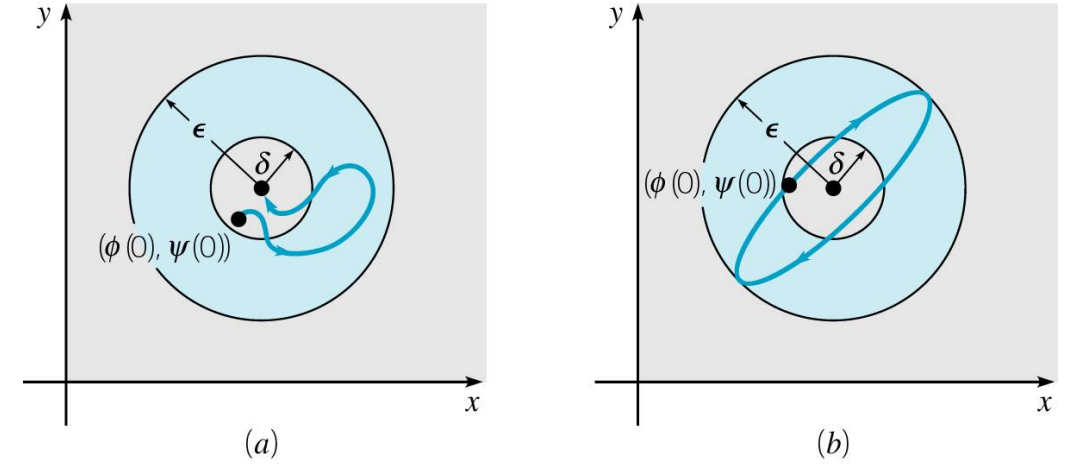
\includegraphics[width=0.55\textwidth]{figure/Lec16f1.PNG}
		\end{figure}
		%
	\end{itemize}
	%
	\section*{Asymptotic stability}
	\begin{itemize}
		\item A critical point $\vb{x}^0$ is said to be asymptotically stable if it is stable and if there exists a $\delta_0 > 0$ such that if a solution $\vb{x} = \phi(t)$ satisfies $||\phi(0) - \vb{x}^0|| < \delta_0$, then $\phi(t) \to \vb{x}^0$ as $t \to \infty$.
		\item Thus trajectories that start “sufficiently close” to $\vb{x}^0$ not only stay close to $\vb{x}^0$ but must eventually approach $\vb{x}^0$ as $t \to \infty$.
		\item This is the case for the trajectory in figure (a) below but not for the one in figure (b) below.
		\item Thus asymptotic stability is a stronger property than stability.
		\item However, note that
		$$
		\lim_{t\to \infty} \phi(t) = \vb{x}^0
		$$
		does not imply stability.
		%
		\begin{figure}[H]
			\centering
				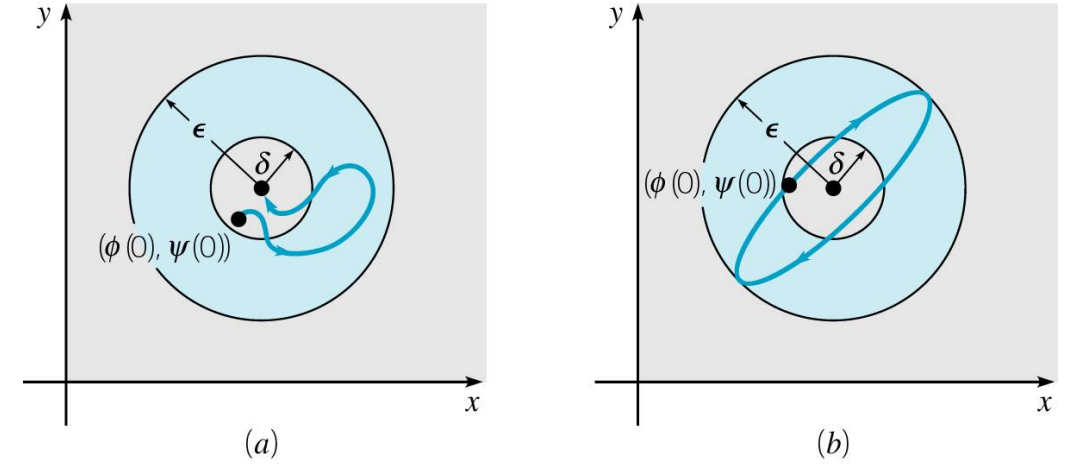
\includegraphics[width=0.55\textwidth]{figure/Lec16f1.PNG}
		\end{figure}
		%
	\end{itemize}
	%
	\section*{Determination of trajectories}
	\begin{itemize}
		\item Consider the autonomous system
		$$
		dx/dt = F(x,y),\ dy/dt = G(x,y)
		$$
		\item It follows that
		$$
		dy/dx = G(x,y)/F(x,y),
		$$
		which is a first order equation in the variables $x$ and $y$.
		\item If we can solve this equation, then the implicit expression for the solution, $H(x,y) = c$, gives an equation for the trajectories of
		$$
		dy/dx = G(x,y)/F(x,y)
		$$
		\item Thus the trajectories lie on the level curves of $H(x,y)$.
		\item Note this approach is applicable only in special cases. 
	\end{itemize}
	%
	\section*{Example 1: Separable equation (1 of 3)}
	\begin{itemize}
		\item Consider the system
		$$
		dx/dt = 4-2y,\ dy/dt = 12-3x^2
		$$
		\item It follows that
		$$
		\frac{dy}{dx} = \frac{12 - 3x^2}{4-2y}\Leftrightarrow (4-2y)dy = (12-3x^2)dx
		$$
		\item The solution of this separable equation is
		$$
		H(x,y) = 4y-y^2-12x+x^3=c
		$$
		\item Note that the equilibrium points are found by solving
		$$
		4-2y = 0,\ 12-3x^2=0,\ \Rightarrow x = \pm 2,\ y = 2
		$$
		and hence $(-2, 2)$ and $(2, 2)$ are the equilibrium points.
	\end{itemize}
	%
	\section*{Example 1: Phase portrait (2 of 3)}
	\begin{itemize}
		\item We have
		$$
		H(x,y)=4y-y^2-12x+x^3=c
		$$
		\item A graph of some level curves of H are given below.
		\item Note that $(-2, 2)$ is a center and $(2, 2)$ is a saddle point.
		\item Also, one trajectory leaves the saddle point (at $t = -\infty$), loops around the center, and returns to the saddle point (at $t = \infty$).
		%
		\begin{figure}[H]
			\centering
				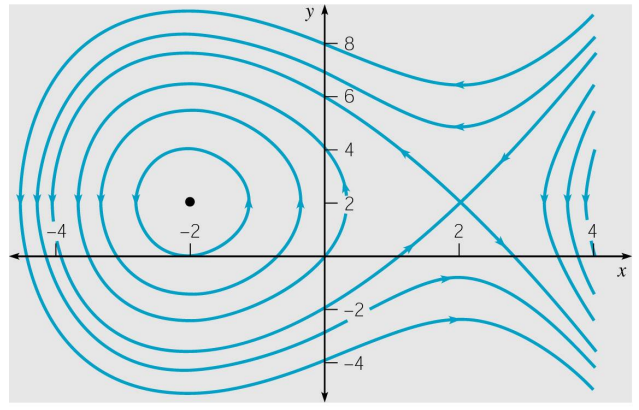
\includegraphics[width=0.55\textwidth]{figure/Lec16f2.PNG}
		\end{figure}
		%
	\end{itemize}
	%
	\section*{Example 1: Phase portrait (2 of 3)}
	%
	\begin{figure}[H]
		\centering
			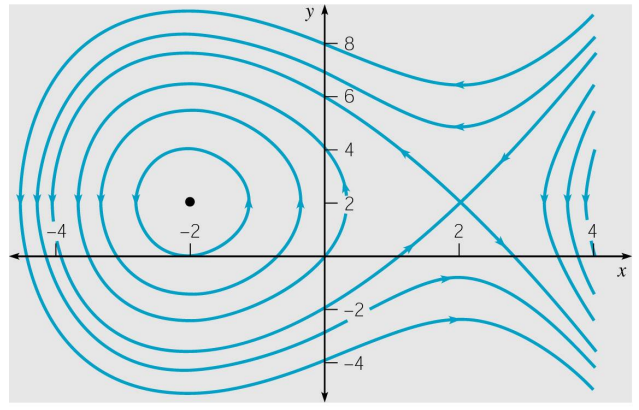
\includegraphics[width=0.75\textwidth]{figure/Lec16f2.PNG}
	\end{figure}
	%
	\section*{Behavior of individual trajectories}
	\begin{itemize}
		\item As $t \to \infty$, each trajectory does one of the following:
		\begin{itemize}
			\item[\labelitemi] approaches infinity;
			\item[\labelitemi] approaches the critical point $\vb{x} = 0$;
			\item[\labelitemi] repeatedly traverses a closed curve, corresponding to a periodic solution, that surrounds the critical point. 
		\end{itemize}
		\item The trajectories never intersect, and exactly one trajectory passes through each point $(x_0, y_0)$ in the phase plane.
		\item The only solution passing through the origin is $\vb{x} = 0$. Other solutions may approach $(0, 0)$, but never reach it.
		%
		\begin{figure}[H]
			\centering
				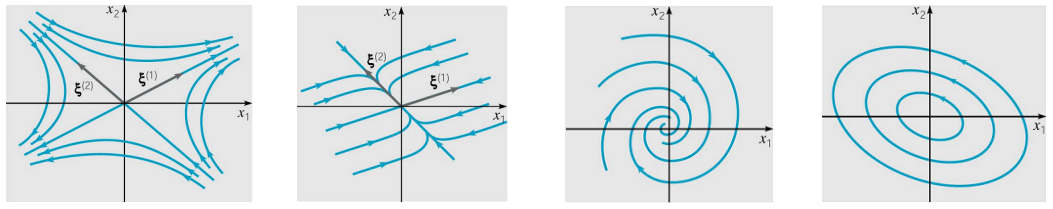
\includegraphics[width=0.85\textwidth]{figure/Lec16f3.PNG}
		\end{figure}
		%
	\end{itemize}
	%
	\section*{Behavior of trajectory sets}

	\begin{itemize}
		\item As $t \to \infty$, one of the following cases holds:
		\begin{itemize}
			\item[\labelitemi] All trajectories approach the critical point $\vb{x} = 0$. This is the case when the eigenvalues are real and negative or complex with negative real part. The origin is either a nodal or spiral sink.
			\item[\labelitemi] All trajectories remain bounded but do not approach the origin, and occur when the eigenvalues are pure imaginary. The origin is a center.
			\item[\labelitemi] Some trajectories, and possibly all trajectories except $\vb{x} = 0$, tend to infinity. This occurs when at least one of the eigenvalues is positive or  has a positive real part. The origin is a nodal source, a spiral source, or a saddle point.
		\end{itemize}
		%
		\begin{figure}[H]
			\centering
				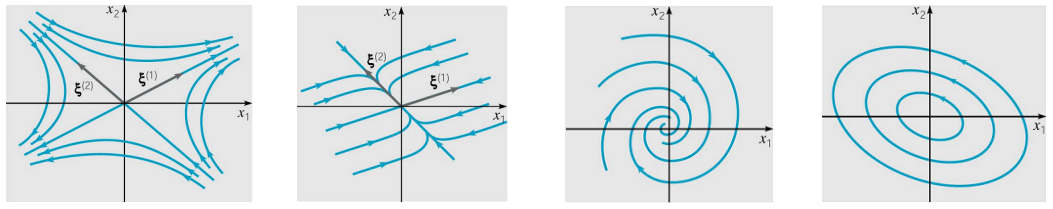
\includegraphics[width=0.85\textwidth]{figure/Lec16f3.PNG}
		\end{figure}
		% 
	\end{itemize}
	%
	\section*{Summary table}
	\begin{itemize}
		\item The following table summarizes the information we have derived about our $2 \times 2$ system $\vb{x}^\prime = \vb{Ax}$, as well as the stability of the equilibrium solution $\vb{x} = 0$.
		%
		\begin{table}[H]
			\centering
			\begin{tabular}{ |l|l|l| } 
			 \hline
			 \textbf{Eigenvalues} & \textbf{Type of Critical Point} & \textbf{Stability}\\
			 \hline
			 $r_1>r_2>0$ & Node & Unstable \\
			 \hline
			 $r_1 < r_2 < 0$ & Node & Asymptotically Stable \\
			 \hline
			 $r_2 < 0 < r_1$ & Saddle Point & Unstable \\ 
			 \hline
			 $r_1 = r_2 > 0$ & Proper or Improper Node & Unstable \\
			 \hline
			 $r_1 = r_2 < 0$ & Proper or Improper Node & Asymptotically Stable \\
			 \hline
			 $r_1,r_2 = \lambda \pm i\mu$ & Spiral Point &  \\
			 \hline
			 $\lambda > 0$ &  & Unstable \\
			 \hline
			 $\lambda < 0$ &  & Asymptotically Stable \\
			 \hline
			 $r_1 = i\mu, r_2 = -i\mu$ & Center & Stable \\
			 \hline
			\end{tabular}
		\end{table}
		%
	\end{itemize}
	%
	\section*{Almost linear systems}
	\begin{itemize}
		\item We have just given an informal description of the stability properties of the equilibrium solution $\vb{x} = 0$ of the $2 \times 2$ system $\vb{x}^\prime = \vb{Ax}$.
		\item We required $\det A \neq 0$, and hence $\vb{x} = 0$ is the only critical point of the system $\vb{x}^\prime = \vb{Ax}$.
		\item Now that we have precisely defined the concepts of asymptotic stability, stability, and instability, we can restate these results in the Theorem 9.3.1, on the next slide.
	\end{itemize}
	%
	\section*{Theorem 9.3.1}
	\begin{itemize}
		\item The critical point $\vb{x} = 0$ of the $2 \times 2$ linear system $\vb{x}^\prime = \vb{Ax}$ is
		\begin{enumerate}[(1)]
			\item asymptotically stable if the eigenvalues $r_1$ and $r_2$ are real and negative or have negative real part;
			\item stable, but not asymptotically stable, if $r_1$ and $r_2$ are pure imaginary;
			\item unstable if $r_1$ and $r_2$ are real and either is positive, or if they have a positive real part.
		\end{enumerate}
	\end{itemize}
	%
	\section*{Nonlinear systems}
	\begin{itemize}
		\item Consider a nonlinear two-dimensional autonomous system
		$$
		\vb{x}^\prime = f(x)
		$$
		\item Our main object is to investigate the behavior of trajectories of this system near a critical point $\vb{x}^0$.
		\item We do this by approximating the nonlinear system near a critical point $\vb{x}^0$ by an appropriate linear system, whose trajectories are easy to describe.
		\item The crucial question is whether the trajectories of the linear system are good approximations to those of the nonlinear system.
		\item For convenience, assume the critical point is at the origin, $\vb{x}^0 = 0$. This involves no loss of generality, since in general the substitution $\vb{u} = \vb{x}-\vb{x}^0$ shifts the critical point to the origin.
	\end{itemize}
	%
	\section*{Nonlinear and nearly linear systems}
	\begin{itemize}
		\item First, we consider what it means for a nonlinear system to be “close” to a linear system.
		\item Accordingly, suppose that $\vb{x}^\prime = f(x) = \vb{Ax} + g(\vb{x})$.
		\item Assume that $\vb{x} = 0$ is an \textbf{isolated} critical point of this system. This means that there is some circle about the origin within which there are no other critical points.
		\item In addition, assume that $\det \vb{A} \neq 0$, and hence $\vb{x} = 0$ is also an isolated critical point of the system $\vb{x}^\prime = \vb{Ax}$.
		\item For the nonlinear system $\vb{x}^\prime = f(\vb{x})$ to be close to the linear system $\vb{x}^\prime = \vb{Ax}$, we must assume that $g(\vb{x})$ is small.
	\end{itemize}
	%
	\section*{Almost linear systems: vector form}
	\begin{itemize}
		\item Recall: $\vb{x}^\prime = f(\vb{x}) = \vb{Ax} + g(\vb{x})$, where $g(\vb{x})$ is small.
		\item More precisely, assume the components of $g$ have continuous first partial derivatives and satisfy the limit condition
		$$
		\lim_{x\to 0}\frac{||g(\vb{x})||}{||\vb{x}||} = 0
		$$
		\item Thus $||g(\vb{x})||$ is small compared to $||\vb{x}||$ near the origin.
		\item Such a system is called an \textbf{almost linear system} in the neighborhood of the critical point $\vb{x} = 0$.
	\end{itemize}
	%
	\section*{Almost linear systems: scalar form}
	\begin{itemize}
		\item Recall: $\vb{x}^\prime = f(\vb{x}) = \vb{Ax} + g(\vb{x})$, where
		$$
		\lim_{x\to 0} = \frac{||g(\vb{x})||}{||\vb{x}||} = 0
		$$
		\item In scalar form, if we let
		$$
		\vb{x} =
		\begin{pmatrix}
			x\\
			y
		\end{pmatrix},\ g(\vb{x}) =
		\begin{pmatrix}
			g_1(x,y)\\
			g_2(x,y)
		\end{pmatrix}
		$$
		then
		$$
		||\vb{x}|| = \sqrt{x^2 + y^2} = r,\ ||g(\vb{x})|| = \sqrt{g_1^2(x,y)+g_2^2(x,y)},
		$$
		and the corresponding limit condition is
		$$
		\lim_{r\to 0}\frac{g_1(x,y)}{r} = 0\ \text{and}\ \lim_{r\to 0}\frac{g_2(x,y)}{r} = 0
		$$
	\end{itemize}
	%
	\section*{General nonlinear system (1 of 3)}
	\begin{itemize}
		\item Consider the general nonlinear system $\vb{x}^\prime = f(\vb{x})$, or
		$$
		x^\prime = F(x,y),\ y^\prime = G(x,y)
		$$
		\item We will show that this system is almost linear near a critical point $(x_0, y_0)$ whenever the functions $F$ and $G$ have continuous partial derivatives up to order 2.
		\item To see this, we use Taylor expansions about the point $(x_0, y_0)$ to write $F(x,y)$ and $G(x,y)$ in the form
		\begin{align*}
			F(x,y) &= F(x_0, y_0) + F_x(x_0, y_0)(x-x_0)+F_y(x_0, y_0)(y-y_0) + \eta_1(x,y),\\
			G(x,y) &= G(x_0, y_0) + G_x(x_0, y_0)(x-x_0)+G_y(x_0, y_0)(y-y_0) + \eta_2(x,y)
		\end{align*}
		where
		$$
		\lim_{(x,y)\to (x_0,y_0)}\frac{\eta_1(x,y)}{\sqrt{(x-x_0)^2 + (y-y_0)^2}} = \lim_{(x,y)\to (x_0,y_0)}\frac{\eta_2 (x,y)}{\sqrt{(x-x_0)^2+(y-y_0)^2}} = 0
		$$
	\end{itemize}
	\section*{General nonlinear system (2 of 3)}
	\begin{itemize}
		\item We have $F(x,y)$ and $G(x,y)$ in the form
		\begin{align*}
			F(x,y) &= F(x_0, y_0) + F_x(x_0, y_0)(x-x_0)+F_y(x_0, y_0)(y-y_0) + \eta_1(x,y),\\
			G(x,y) &= G(x_0, y_0) + G_x(x_0, y_0)(x-x_0)+G_y(x_0, y_0)(y-y_0) + \eta_2(x,y)
		\end{align*}
		\item Since $(x_0, y_0)$ is a critical point, $F(x_0, y_0) = G(x_0, y_0) = 0$. Also, note that $dx/dt = d(x - x0)/dt$ and $dy/dt = d(y - y_0)/dt$.
		\item Thus the original system of equations
		$$
		x^\prime = F(x,y),\ y^\prime = G(x,y)
		$$
		reduces to
		$$
		\frac{d}{dt}
		\begin{pmatrix}
			x-x_0\\
			y-y_0
		\end{pmatrix}=
		\begin{pmatrix}
			F_x(x_0, y_0) & F_y(x_0, y_0)\\
			G_x(x_0, y_0) & G_y(x_0, y_0)
		\end{pmatrix}
		\begin{pmatrix}
			x-x_0\\
			y-y_0
		\end{pmatrix} +
		\begin{pmatrix}
			\eta_1(x,y)\\
			\eta_2(x,y)
		\end{pmatrix}
		$$
	\end{itemize}
	%
	\section*{General nonlinear system (3 of 3)}
	\begin{itemize}
		\item Thus our system of equations can be written as
		$$
		\frac{d}{dt}
		\begin{pmatrix}
			x-x_0\\
			y-y_0
		\end{pmatrix}=
		\begin{pmatrix}
			F_x(x_0, y_0) & F_y(x_0, y_0)\\
			G_x(x_0, y_0) & G_y(x_0, y_0)
		\end{pmatrix}
		\begin{pmatrix}
			x-x_0\\
			y-y_0
		\end{pmatrix} +
		\begin{pmatrix}
			\eta_1(x,y)\\
			\eta_2(x,y)
		\end{pmatrix}
		$$
		\item In vector notation,
		$$
		\frac{d \vb{u}}{dt} = \frac{d \vb{f}}{d \vb{x}}(\vb{x}^0)\vb{u} + \vb{\eta(\vb{x})},\ \text{where}\ \vb{u}(x) =
		\begin{pmatrix}
			x-x_0\\
			y-y_0
		\end{pmatrix},\ \eta(\vb{x}) =
		\begin{pmatrix}
			\eta_1(x,y)\\
			\eta_2(x,y)
		\end{pmatrix}
		$$
		\item Thus if F and G are twice differentiable, then the nonlinear system of equations $\vb{x}^\prime = f(\vb{x})$ is almost linear, and the linear system that approximates the nonlinear system is given by
		$$
		\frac{d}{dt}
		\begin{pmatrix}
			u_1\\
			u_2
		\end{pmatrix}=
		\begin{pmatrix}
			F_x(x_0, y_0) & F_y(x_0,y_0)\\
			G_x(x_0,y_0) & G_y(x_0,y_0)
		\end{pmatrix}
		\begin{pmatrix}
			u_1\\
			u_2
		\end{pmatrix},\ \text{where}\ 
		\begin{pmatrix}
			u_1\\
			u_2
		\end{pmatrix}=
		\begin{pmatrix}
			x-x_0\\
			y-y_0
		\end{pmatrix}
		$$
	\end{itemize}
	%
	\section*{Theorem 9.3.2}
	\begin{itemize}
		\item Consider the almost linear system $\vb{x}^\prime = \vb{Ax} + g(\vb{x})$. Let $r_1$ and $r_2$ be the eigenvalues of $\vb{A}$. Then the type and stability of the critical point $(0,0)$ of the linear system $\vb{x}^\prime = \vb{Ax}$ and the almost linear system $\vb{x}^\prime = \vb{Ax} + g(\vb{x})$ are as given in the table below.
		%
		\begin{table}[H]
			\begin{adjustbox}{width=\columnwidth,center}
			\begin{tabular}{ |l|l|l|l|l| } 
				\hline
				& \multicolumn{2}{|c|}{Linear System} & \multicolumn{2}{|c|}{Almost Linear System}\\
				\hline
				\textbf{Eigenvalues}&\textbf{Type}&\textbf{Stability}&\textbf{Type}&\textbf{Stability}\\
				\hline
				$r_1>r_2>0$ & Node & Unstable & Node & Unstable\\
				\hline
				$r_1 < r_2 < 0$ & Node & Asymptotically Stable & Node & Asymptotically Stable\\
				\hline
				$r_2 < 0 < r_1$ & Saddle Point & Unstable & Saddle Point & Unstable\\ 
				\hline
				$r_1 = r_2 > 0$ & Proper or Improper Node & Unstable & Node or Spiral Point & Unstable\\
				\hline
				$r_1 = r_2 < 0$ & Proper or Improper Node & Asymptotically Stable & Node or Spiral Point & Asymptotically Stable\\
				\hline
				$r_1,r_2 = \lambda \pm i\mu$ & & & &\\
				\hline
				$\lambda > 0$ & Spiral Point & Unstable & Spiral Point & Unstable\\
				\hline
				$\lambda < 0$ & Spiral Point & Asymptotically Stable & Spiral Point & Asymptotically Stable\\
				\hline
				$r_1 = i\mu, r_2 = -i\mu$ & Center & Stable & Center or Spiral Point & Indeterminate\\
				\hline
			\end{tabular}
			\end{adjustbox}
		\end{table}
		%
	\end{itemize}
	%
	\section*{Theorem 9.3.2 Discussion (1 of 2)}
	\begin{itemize}
		\item Since the nonlinear term $g(\vb{x})$ is small compared to the linear term $\vb{Ax}$ when $\vb{x}$ is small, we hope that the trajectories of the linear system $\vb{x}^\prime = \vb{Ax}$ are good approximations to those of the nonlinear system, at least near the origin.
		\item Theorem 9.3.2 states that this is true in many but not all cases. For small $\vb{x}$, the nonlinear terms are small and do not affect the stability and type of critical point as determined by the linear term, except in two sensitive cases: $r_1$ and $r_2$ pure imaginary, and $r_1$ and $r_2$ real and equal.
		\item As we have seen earlier, small changes in eigenvalues can alter the type and stability of the critical point for a linear system, but only in these two cases. Thus a small nonlinear term might have a similar effect for these two cases as well;
	\end{itemize}
	\section*{Theorem 9.3.2 Discussion (2 of 2)}
	\begin{itemize}
		\item Even if the critical point is of the same type as that of the linear system, the trajectories of the almost linear system may be much different in appearance than for the linear system, except very near the critical point.
		\item However, it can be shown that the slopes at which the trajectories “enter” or “leave” the critical point are given correctly by the linear equation.
		%
		\begin{figure}[H]
			\centering
				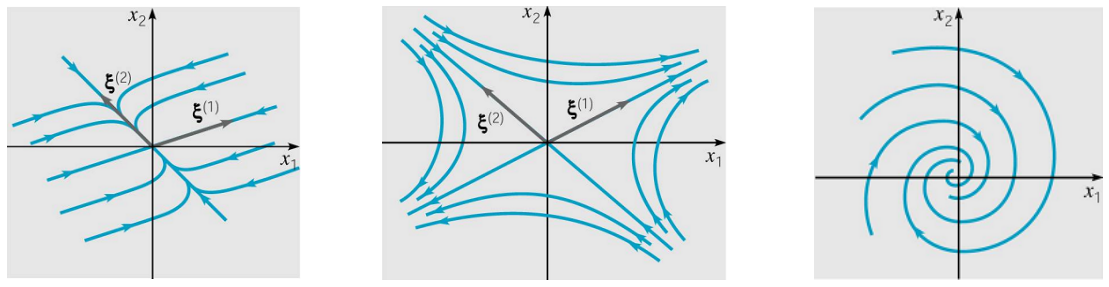
\includegraphics[width=0.85\textwidth]{figure/Lec16f4.PNG}
		\end{figure}
		%
	\end{itemize}
\end{document}